\usetikzlibrary{calc,positioning}
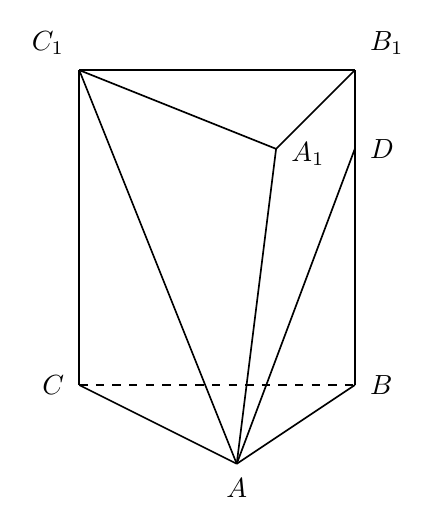
\begin{tikzpicture}[x=1cm,y=1cm,line width=.6pt,font=\normalsize,
 geometry edge/.style={solid,line width=.6pt,draw=black},
 geometry label/.style={font=\normalsize,inner sep=1.5pt,outer sep=4pt,fill=white,draw=none}]

\coordinate (C1) at (1,5);
\coordinate (B1) at (4.5,5);
\coordinate (A1) at (3.5,4);
\coordinate (C) at (1,1);
\coordinate (B) at (4.5,1);
\coordinate (A) at (3,0);
\coordinate (D) at (4.5,4);
\draw[geometry edge] (C1)--(B1);
\draw[geometry edge] (C1)--(A1);
\draw[geometry edge] (B1)--(A1);
\draw[geometry edge] (C1)--(C);
\draw[geometry edge] (B1)--(B);
\draw[geometry edge] (A1)--(A);
\draw[geometry edge] (C1)--(A);
\draw[geometry edge] (A)--(B);
\draw[geometry edge] (A)--(C);
\draw[geometry edge] (A)--(D);
\draw[geometry edge,dashed] (C)--(B);
\node[geometry label,above left] at (C1) {$C_{1}$};
\node[geometry label,above right] at (B1) {$B_{1}$};
\node[geometry label,right,fill=none,xshift=0.00bp,yshift=-2.00bp] at (A1) {$A_{1}$};
\node[geometry label,left] at (C) {$C$};
\node[geometry label,right] at (B) {$B$};
\node[geometry label,below] at (A) {$A$};
\node[geometry label,right] at (D) {$D$};
\end{tikzpicture}
